\documentclass[a4paper,UTF8]{ctexart}

\usepackage{amsmath, amsthm, amssymb, amsfonts, hyperref, mathrsfs}%美国数学学会的包+?
\usepackage{geometry} %控制界面
\usepackage{bookmark}
\usepackage{fancyhdr} % header & footer
\usepackage{appendix} % 附录
\usepackage{tikz} %作图
\usepackage{graphicx} %插入图片的宏包
\usepackage{float} %设置图片浮动位置的宏包
%\usepackage{subfigure} %插入多图时用子图显示的宏包
\usepackage{listings} %引用代码
\usepackage{physics,mathtools} %物理数学工具
\usepackage{comment}
\usepackage{framed}
\usepackage{caption}
\usepackage{subcaption}
\geometry{top=2.5cm,bottom=2.5cm,left=2.5cm,right=2.5cm} % 布局要求
\pagestyle{fancy} % fancy分格
\fancyhf{} % 清除所有页眉页脚
\renewcommand\headrulewidth{0.6pt}
\renewcommand\footrulewidth{0.6pt}
% font
\setCJKmainfont{Noto Serif CJK SC}[BoldFont={Noto Serif CJK SC Bold}, ItalicFont=]
\lhead{何金铭 PB21020660$\mid$座位号:4}
\chead{双光子HOM干涉实验预习报告}
\rhead{\thepage}
\lfoot{2024.4.9}
\rfoot{USTC}
%\bibliographystyle{plain} % 引用样式
\everymath{\displaystyle} % display
%============================================================

\begin{document}

\begin{center}
    \textbf{\Large 双光子HOM干涉实验预习报告}
    \par \text{\large 何金铭 PB21020660}
\end{center}

\section{实验目的}

\begin{enumerate}
    \item 通过实验熟悉产生HOM干涉的基本条件。
    \item 熟悉自发参量下转换过程,了解光子产生率的依赖因素,符合信噪比的依赖因素
    \item 掌握HOM干涉曲线的测量、干涉可见度计算、光子带宽计算和误差分析。
\end{enumerate}

\section{实验原理}

\subsection{HOM干涉的原理}

如下图所示,当两个光子沿路径a和b入射到分束器时,其出射光子的可能情况有四种,
即两个光子同时透射和反射,其中一个光子透射另一个光子反射,
分别对应下图中的四种光子出射分布情况。

\begin{figure}[H]
    \centering
    \begin{minipage}[b]{0.9\textwidth}
        \centering
        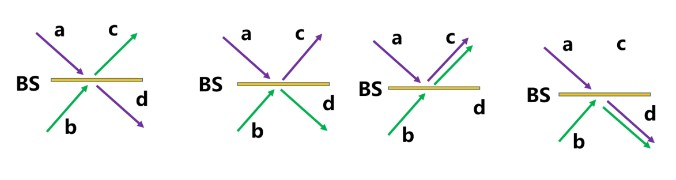
\includegraphics[width=0.9\textwidth]{./fig2.jpg}
        \caption{两光子入射到分束器上有四种可能的输出状态}
    \end{minipage}
\end{figure}

在光子数表象下,出射光子的量子态可以写成:

\begin{equation}
    \ket{\Phi}_{out} = (R-T) \ket{1_c,1_d} + i\sqrt{2RT}\ket{2_c,0_d} + \ket{0_c,2_d}
\end{equation}

其中{\bfseries{符合计数}}指:{\bfseries{c,d同时有光子出射}}

若假设我们的干涉滤波器的滤波函数是高斯型函数$g(\tau) = \exp{(-\Delta \omega \tau^2 /2)}$。最后得到复合计数的表达式为:

\begin{equation}
    N_{cd} = \kappa (T^2+R^2)[1-\frac{2RT}{T^2+R^2}\exp{(-\Delta \omega \delta \tau)}]
\end{equation}

可以很明显的看出,复合计数在相对延迟为零时的符合计数最低,形成一个低谷,低谷的半高宽度与光子的带宽$\Delta \omega$有关。
得到的结果如下图所示:

\begin{figure}[H]
    \centering
    \begin{minipage}[b]{0.9\textwidth}
        \centering
        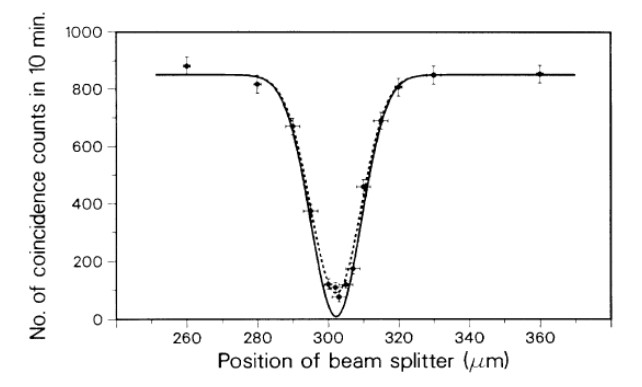
\includegraphics[width=0.9\textwidth]{./fig3.jpg}
        \caption{第一次HOM干涉曲线}
    \end{minipage}
\end{figure}

\subsection{自发参量下转换过程}

在二阶非线性过程中,一个高频光子会以一定的概率劈裂成信号光子和闲频光子,相互作用的哈密顿量为:

\begin{equation}
    \hat{H} = \hbar \xi (\hat{a}_s^{\dagger}\hat{a}_i^{\dagger}+H.C.)
\end{equation}

于粒子数表象下自发参量产生的态的表达式如下:

\begin{equation}
    \ket{\Phi} = \exp{(-\frac{i\hat{H}t}{\hbar})}\ket{0,0} = \ket{0,0} + \kappa\ket{1,1} + \frac{\kappa^2}{2}\ket{2,2}
\end{equation}

对于单色高斯泵浦光,产生的光子使用单模光纤收集和探测,其光子的收集概率的表达式如下:

\begin{equation}
    P_{si} \approx \frac{64\pi^3\hbar c \varepsilon n_s n_i}{\varepsilon_0 n_p \abs{n_s'-n_i'}}(\frac{\chi_{eff}^2}{\lambda_s \lambda_i})^2 \frac{\arctan\xi}{A^{+}B^{+}} N_p
\end{equation}

\begin{equation}
    P_{si} \approx \frac{64\pi^3\hbar c \varepsilon n_s n_i}{\varepsilon_0 n_p \abs{n_s'-n_i'}}(\frac{\chi_{eff}^2}{\lambda_s \lambda_i})^2 \frac{\arctan\frac{B_s}{A_s}\xi_s}{A_s B_s} N_p
\end{equation}

$n_s,n_i$为信号和闲频光子的折射率,$n_p$为泵浦光的折射率;$n_s',n_i'$为信号光子和闲频光子折射率对圆频率的微分;
$\chi_{eff}^2$是有效非线性系数;$\lambda_s,\lambda_i$为信号与闲频光子的波长;$\varepsilon$为光场直接的模式交叠系数;
$\xi,A^{+},B^{+}$是聚焦因子有关的参数;$N_p$为泵浦光子数。
可以很明显的看出光子的收集概率与泵浦数成正比,即正比于泵浦光的功率。

\subsection{光子符合信噪比与功率的关系}

光子符合测量信噪比的定义为有效符合的大小与延迟远离中心的符合大小
的比值,其定义和依赖的参数如下:
\begin{equation}
    CAR = \frac{R_{cc} + R_{acc}}{R_{acc}} = \frac{\mu_c \alpha_s \alpha_i}{[(\mu_c +\mu_{sn})\alpha_s + d_s][(\mu_c+\mu_{in})\alpha_i+d_i]}+1
\end{equation}

其中$R_{cc}$代表符合计数率,$R_{acc}$代表暗符合计数率;$\mu_c$为每脉冲产生一对光子的概率;
$\alpha_s,\alpha_i$表示光子的收集探测效率,包括传输效率和探测效率;$\mu_{sn},\mu_{in}$为信号与闲频信道产生的不可去除的噪声光子;
$d_s,d_i$为信号与闲频信道单光子探测器没脉冲的暗计数概率。
对于晶体中的自发参量过程,一般$\mu_{sn},\mu_{in}=0$。典型的CAR曲线如下图所示。

\begin{figure}[H]
    \centering
    \begin{minipage}[b]{0.9\textwidth}
        \centering
        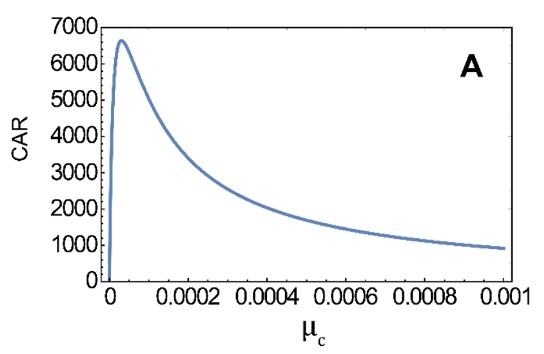
\includegraphics[width=0.9\textwidth]{./fig4.jpg}
        \caption{复合与暗符合比值与光子产生率的关系}
    \end{minipage}
\end{figure}

\section{实验内容}

实验采用的光路图如下:

\begin{figure}[H]
    \centering
    \begin{minipage}[b]{0.9\textwidth}
        \centering
        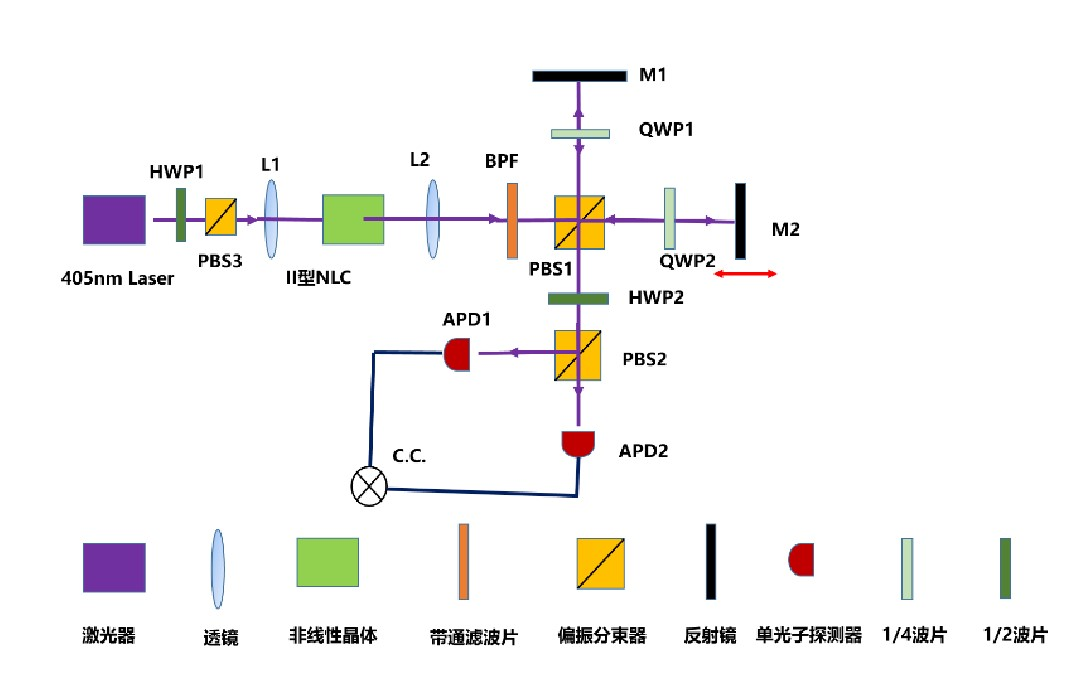
\includegraphics[width=0.9\textwidth]{./fig1.jpg}
        \caption{采用的HOM干涉实验光路图}
    \end{minipage}
\end{figure}

\subsection{光子单路计数和复合计数与泵浦功率的关系实验}

将偏振迈克尔逊干涉仪中的两个四分之一波片的光轴转动45度,使得两路光子都从另外一个端口输出,
转动PBS2前的半波片HWP2,使得半波片处于光轴与垂直偏振重叠的位置,
这样两路光子的偏振依然保持正交不变,
两路探测器探测到的是无干涉情况下的光子单路计数和符合。

\subsection{符合信噪比与泵浦功率的关系}

实验中可以通过改变405nm的泵浦功率,记录不同功率下的有效符合和暗符合的大小,
并且计算该功率下的CAR值。其中,暗符合需要在远离符合窗口的延迟下获得。

\subsection{HOM干涉曲线测量}

在进行HOM干涉实验测量时,需要将偏振分束器PBS2的前的半波片的角度转动22.5度,
使得两个光子以相等的概率在分束器上进行干涉,通过移动反射镜M2的一维平移台,
记录下不同位置的符合计数率,并且记录下来,然后对采集的数据进行画图和拟合分析。

\end{document}